\documentclass[9pt]{beamer}

% Configuration {{{
\usepackage[utf8]{inputenc}
\usepackage[T2A]{fontenc} % T1 for English
\usepackage[english, russian]{babel}

\usepackage{mathtools}
\usepackage{graphicx}
\usepackage[multidot]{grffile}
\usepackage[labelsep=period]{caption}

\setbeamertemplate{caption}[numbered]
\setbeamertemplate{navigation symbols}{}
\usefonttheme[onlymath]{serif}
\usepackage{DejaVuSansCondensed} % helvet for English
\usetheme{Madrid}

\linespread{1.2}
% }}}

\title[Рассеяние на $\delta$-потенциале]{Коэффициент отражения от одиночного и двойного $\delta$-потенциала}
\author{Керим Гусейнов}
\institute[]{МГУ им. М. В. Ломоносова \\ Кафедра общей ядерной физики}
\date{\today}

\begin{document}

\frame[plain]{
	\titlepage
}

\frame{% Shroedinger and Stitching {{{
	\frametitle{Одиночный $\delta$-потенциал. Уравнение Шредингера}
	$$ \psi''(x) + \frac{2m}{\hbar^2}\Big(E - V(x)\Big) \psi(x) = 0,
	\qquad V(x) = v_0\,\delta(x) $$
	$$
	\begin{aligned}
		x < 0: \qquad & \psi''(x) + \frac{2mE}{\hbar^2} \psi(x) = 0 \\
		x > 0: \qquad & \psi''(x) + \frac{2mE}{\hbar^2} \psi(x) = 0
	\end{aligned}
	$$

	$$\psi(x) = \left\{
		\begin{array}{lc}
			e^{ikx} + B e^{-ikx}, & x < 0, \\
			C e^{ikx}, & x > 0,
		\end{array}
		\right.
		\qquad k = \sqrt{\frac{2mE}{\hbar^2}}
	$$

	Изменяются условия сшивки

	$$\int_{-0}^{+0} \left(\psi''(x) + \frac{2m}{\hbar^2}\Big(E - v_0\,\delta(x)\Big) \psi(x)\right) \mathrm{d} x = 0 $$
	$$\psi'(+0) - \psi'(-0) - \frac{2mv_0}{\hbar^2} \psi(0) = 0 $$
	$$\psi(-0) = \psi(+0) = \psi(0)$$
}% }}}

\frame{% R and D for single {{{
	\frametitle{Одиночный $\delta$-потенциал. Отражение и прохождение}

	\begin{center}
		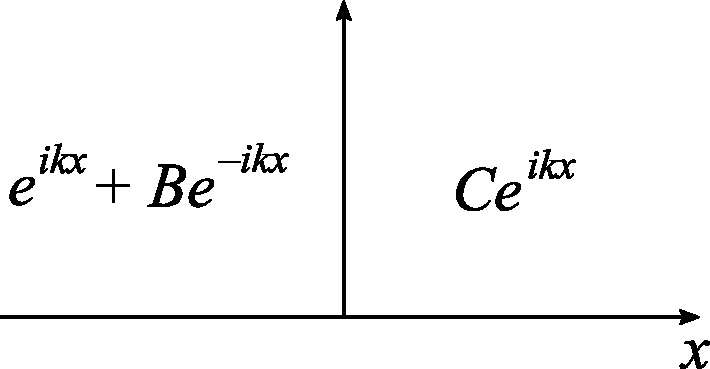
\includegraphics[width=.5\linewidth]{figures/single-delta}
	\end{center}
	
	\vfill

	\begin{columns}
		\column{.49\linewidth}{
			$$ k = \sqrt{\frac{2mE}{\hbar^2}}, \quad k_0 = \frac{2mv_0}{\hbar^2} $$

			$$\begin{aligned} 1 + B &= C\\ ikC - (ik - ikB) &= k_0 C \end{aligned} $$

	$$ B = \frac{k_0}{2ik - k_0}, \qquad C = \frac{2ik}{2ik - k_0} $$
		}

		\column{.49\linewidth}{
	$$ R = |B|^2 = \frac{k_0^2}{{k_0^2 + 4k^2}} $$
	$$ D = |C|^2 = \frac{4k^2}{{k_0^2 + 4k^2}} $$
		}
	\end{columns}

	\vfill\null
}% }}}

\frame{% Double-delta Figure {{{
	\frametitle{Двойной $\delta$-потенциал}

	\begin{center}
		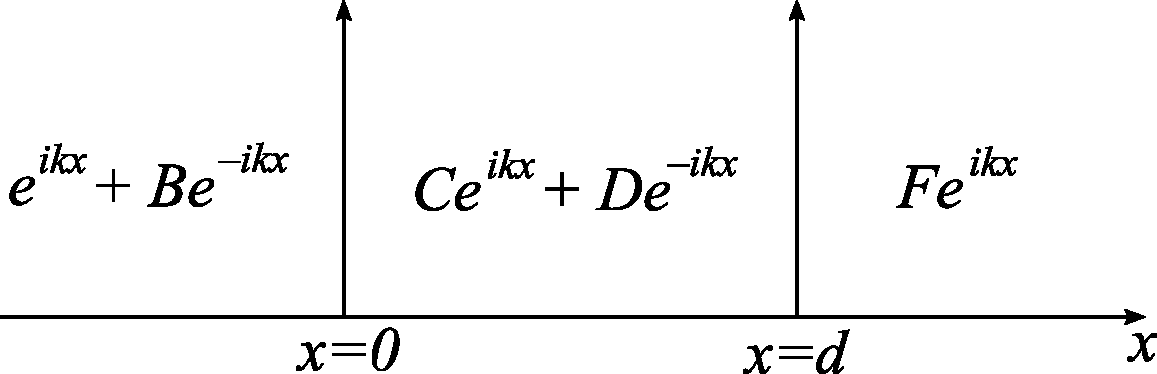
\includegraphics[width=.75\linewidth]{figures/double-delta}
	\end{center}

	\vfill
	\begin{columns}

		\column{.5\linewidth}{
			$$ V(x) = v_0 \, \delta(x) + v_0\, \delta(x-d) $$

			$$\psi(x) = \left\{
				\begin{array}{lc}
					e^{ikx} + B e^{-ikx}, & x < 0 \\
					C e^{ikx} + D e^{-ikx}, & x \in (0, d) \\
					F e^{ikx}, & x > d \\
				\end{array}
			\right.$$
		}

		\column{.6\linewidth}{
		$$ 1 + B = C + D $$
		$$ \frac{k_0}{ik}(1 + B) = C - D - (1 - B) $$
		$$ C e^{ikd} + D e^{-ikd} = F e^{ikd} $$
		$$ \frac{k_0}{ik} F e^{ikd} = F e^{ikd} - (C e^{ikd} - D e^{-ikd})$$
	}

	\end{columns}
}% }}}

\frame{% R = 0 formulas {{{
	\frametitle{Двойной $\delta$-потенциал. Полное прохождение}

	$$ \varkappa = k/k_0, \qquad \varphi = kd = \varkappa\lambda \qquad(\lambda = d/k_0) $$

	$$ B = - \frac{\frac{1}{2}\big(e^{2i\varphi} - 1\big) + i\varkappa \big(e^{2i\varphi} + 1\big)}
	{2\varkappa^2 + 2i\varkappa - \frac{1}{2}\big(e^{2i\varphi} - 1\big)}
	=
	-ie^{i\varphi} \frac{\sin\varphi + 2 \varkappa \cos\varphi}
	{2\varkappa^2 + 2i\varkappa - \frac{1}{2}\big(e^{2i\varphi} - 1\big)}
	$$
	
	$$ F = 1 + B e^{-2i\varphi} + \frac{1+B}{\varkappa} e^{-i\varphi} \sin\varphi $$

	$$ R = |B|^2 = 0 \Rightarrow B = 0 : \qquad -2\varkappa = \tg\varphi = \tg(\varkappa\lambda)$$

	$$ \varkappa \lambda = x, \quad \varkappa = x / \lambda $$
	$$ \boxed{\tg x = - 2 x / \lambda} $$
}% }}}

\frame{% Double-delta R = 0 Plot {{{
	\frametitle{Двойной $\delta$-потенциал. Полное прохождение ($R = 0$, $D = 1$)}

	\centering

	$ \tg x = -2 x /\lambda $

	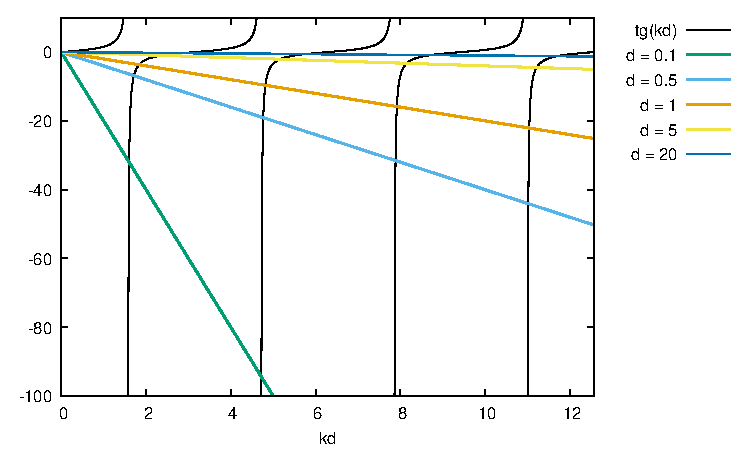
\includegraphics[width=\linewidth]{figures/R-0}
}% }}}

\frame{% R = 1 formulas {{{
	\frametitle{Двойной $\delta$-потенциал. Полное отражение}


	$$ B = -ie^{i\varphi} \frac{\sin\varphi + 2 \varkappa \cos\varphi}
	{2\varkappa^2 + 2i\varkappa - \frac{1}{2}\big(e^{2i\varphi} - 1\big)} $$

	$$ \left(2\varkappa^2 - 2i\varkappa - \frac{1}{2}\big(e^{-2i\varphi} - 1\big)\right) 
	\left(2\varkappa^2 + 2i\varkappa - \frac{1}{2}\big(e^{2i\varphi} - 1\big)\right) =$$
	$$\begin{aligned}
		=& 4\varkappa^4 + 2\varkappa^2 + \frac{1}{4}\big(e^{2i\varphi} - 1\big)\big(e^{-2i\varphi} - 1\big) 
	-4i\varkappa^3 + 4i\varkappa^3 - \varkappa^2\big(e^{-2i\varphi} - 1\big) \\
		& - \varkappa^2\big(e^{2i\varphi} - 1\big)  -i\varkappa\big(e^{-2i\varphi} - 1\big) +i\varkappa\big(e^{2i\varphi} - 1\big)
		\\
		=& 4\varkappa^4 + 4\varkappa^2 + \sin^2\varkappa + \varkappa(2 - 2\cos(2\varphi)) - 2\varkappa\sin(2\varphi)
	\end{aligned}$$

	$$ R = |B|^2 = \frac{(\sin\varphi + 2\varkappa\cos\varphi)^2}
	{4\varkappa^4 + 4\varkappa^2(1 + \sin^2\varphi) + \sin^2\varkappa - 2\varkappa\sin(2\varphi)}  = 1$$

	$$ \sin^2\varphi + 4\varkappa^2\cos^2\varphi + 2\varkappa\sin(2\varphi) = 4\varkappa^4 + 4\varkappa^2(1 + \sin^2\varphi) + \sin^2\varkappa - 2\varkappa\sin(2\varphi) $$
	$$ 4\varkappa^4 + 8\varkappa^2\sin^2\varphi - 4\varkappa\sin(2\varphi) = 0 \qquad
	\boxed{\varkappa^3 + 2\varkappa\sin^2\varphi - \sin(2\varphi) = 0}$$
}% }}}

\frame{% Double-delta R = 1 Plot {{{
	\frametitle{Двойной $\delta$-потенциал. Полное отражение ($R = 1$, $D = 0$)}
	\centering

	$x^3/\lambda^3 + 2x/\lambda\,\sin^2x - \sin(2x) = 0$

	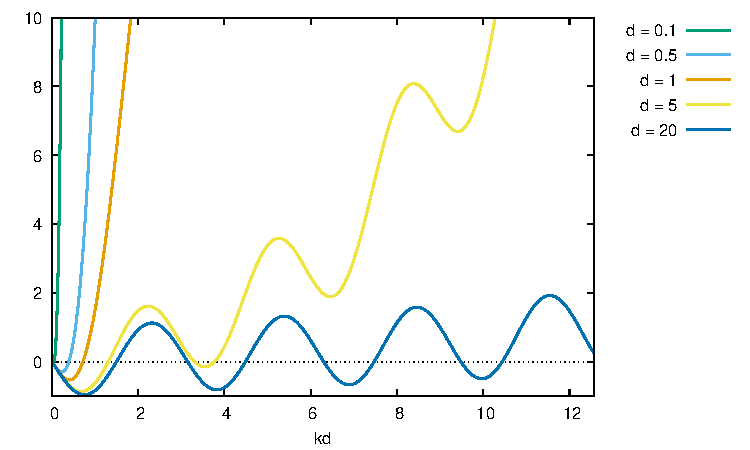
\includegraphics[width=\linewidth]{figures/R-1}
}% }}}

\end{document}
